% !TEX root = main.tex
\section{System Specifications}
\label{sec:specifications}
The proposed radio communication system is designed to switch between QPSK and QAM-16 modulation in order to obtain adaptable sound quality. The system use the 2.4GHz ISM band with a carrier frequency of 2.415GHz and 2.455GHz for the data path and BER path respectively. The system is designed for a transmission distance of 5 meter in an indoor environment. 

Some key system specifications are listed in table \ref{tab:specs_data} and \ref{tab:specs_ber}. Table \ref{tab:specs_data} shows the parameters for the data path, for low / high data rate transmission. Table \ref{tab:specs_ber} shows parameters for the simpler BER path. 
% !TEX root = main.tex
% Table generated by Excel2LaTeX from sheet 'specs'
\begin{table*}[htbp]
  \centering
  \caption{System specifications}
    \begin{tabular}{lcccrr}
    \rowcolor[rgb]{ 0,  0,  0} \multicolumn{1}{c}{\textcolor[rgb]{ 1,  1,  1}{\textbf{System Variables}}} & \textcolor[rgb]{ 1,  1,  1}{\textbf{Variable}} & \textcolor[rgb]{ 1,  1,  1}{\textbf{Units}} & \textcolor[rgb]{ 1,  1,  1}{\textbf{Equation}} & \multicolumn{2}{c}{\textcolor[rgb]{ 1,  1,  1}{\textbf{Value}}} \\
    \rowcolor[rgb]{ 0,  0,  0} \textcolor[rgb]{ 1,  1,  1}{} & \textcolor[rgb]{ 1,  1,  1}{} & \textcolor[rgb]{ 1,  1,  1}{} & \textcolor[rgb]{ 1,  1,  1}{} & \multicolumn{1}{c}{\textcolor[rgb]{ 1,  1,  1}{\textbf{Low Data Rate}}} & \multicolumn{1}{c}{\textcolor[rgb]{ 1,  1,  1}{\textbf{High Data Rate}}} \\
    Frequency & $f_0$ & MHz   &       & 2415  & 2415 \\
    Modulation &       &       &       & \multicolumn{1}{l}{QPSK} & \multicolumn{1}{l}{QAM64} \\
    Bit per symbol  & m     &       &       & 2     & 6 \\
    Sound sampling rate & $f_s$ & Hz    &       & 11025 & 22050 \\
    Bits per sound sample & $b_s$ & bits  &       & 8     & 12 \\
    Sound datarate & $R_{ss}$ & kbits/s & $f_s \cdot b_s$ & 88,2  & 264,6 \\
    Channel coding &       &       &       & \multicolumn{1}{l}{Hamming (4,7)} & \multicolumn{1}{l}{Hamming (4,7)} \\
    Channel coded data rate &       & bits  & $R_ss \cdot 7/4$ & 154,35 & 463,05 \\
    \rowcolor[rgb]{ 0,  0,  0} \textcolor[rgb]{ 1,  1,  1}{\textbf{Packet Parameters}} & \textcolor[rgb]{ 1,  1,  1}{} & \textcolor[rgb]{ 1,  1,  1}{} & \textcolor[rgb]{ 1,  1,  1}{} & \multicolumn{2}{c}{\textcolor[rgb]{ 1,  1,  1}{}} \\
    Packet header size  &       & bits  &       & \headerBits    & \headerBits \\
    Packet data length &       & symbols &       & \packetSataSymbols   & \packetSataSymbols \\
    Packet size &       & bits  &       & \packetDataBitsQPSK   & \packetDataBitsQPSK \\
    \rowcolor[rgb]{ 0,  0,  0} \textcolor[rgb]{ 1,  1,  1}{\textbf{Frame Parameters}} & \textcolor[rgb]{ 1,  1,  1}{} & \textcolor[rgb]{ 1,  1,  1}{} & \textcolor[rgb]{ 1,  1,  1}{} & \multicolumn{2}{c}{\textcolor[rgb]{ 1,  1,  1}{}} \\
    Training sequence type &       &       &       & \multicolumn{1}{l}{Barker} & \multicolumn{1}{l}{Barker} \\
    Training sequence length &       & symbols &       & \barkerSymbols    & \barkerSymbols \\
    Training sequence size bits &       & bits  &       & \frameSizeBitsQPSK    & \frameSizeBitsQAM \\
    Frame size &       & bits  &       & 319   & 935 \\
    \rowcolor[rgb]{ 0,  0,  0} \textcolor[rgb]{ 1,  1,  1}{\textbf{Burst Parameters}} & \textcolor[rgb]{ 1,  1,  1}{} & \textcolor[rgb]{ 1,  1,  1}{} & \textcolor[rgb]{ 1,  1,  1}{} & \multicolumn{2}{c}{\textcolor[rgb]{ 1,  1,  1}{}} \\
    Guard period &       & symbols &       & \guardSymbols     & \guardSymbols \\
    Burst size &       & bits  &       & \burstSizeBitsQPSK   & \burstSizeBitsQAM \\
    \rowcolor[rgb]{ 0,  0,  0} \textcolor[rgb]{ 1,  1,  1}{\textbf{Transmission Characteristics}} & \textcolor[rgb]{ 1,  1,  1}{} & \textcolor[rgb]{ 1,  1,  1}{} & \textcolor[rgb]{ 1,  1,  1}{} & \textcolor[rgb]{ 1,  1,  1}{} & \textcolor[rgb]{ 1,  1,  1}{} \\
    System bit rate & $R_b$ & kbits/s &       & \systemBitRateQPSK & \systemBitRateQAM \\
    Symbol rate & $R_s$ & ksymbols/s &       & \symbolRateQPSK & \symbolRateQAM \\
          &       &       &       &       &  \\
    Pulse shaping filter &       &       &       & \multicolumn{1}{l}{root raised cosine} & \multicolumn{1}{l}{root raised cosine} \\
    Pulse shaping filter parameter & $\alpha$ &       &       & 0,3   & 0,3 \\
    \textbf{Minimum signal bandwidth} & $\Delta f$ & kHz   &       & \textbf{\minBWQPSK} & \textbf{\minBWQAM} \\
    \end{tabular}%
  \label{tab:addlabel}%
\end{table*}%


The burst format for the transmitted data is shown in figure \ref{fig:burst_format}. The bursts are different when using QPSK and QAM-16 modulation, because the same number of training symbols maps to a different number of bits. The data packets (a and b) is transmitted continuously with the indicated guard period. The BER packets is very small compared to the data packets, and is only transmitted ones per received data packet. Thus no guard period is specified for these packets. 

Note that this system is implemented with constant payload size, which means that the packet rate is varied when the data rate changes.

% !TEX root = main.tex
\begin{figure} 
    \centering
  \subfloat[QPSK data packet\label{1a}]{%
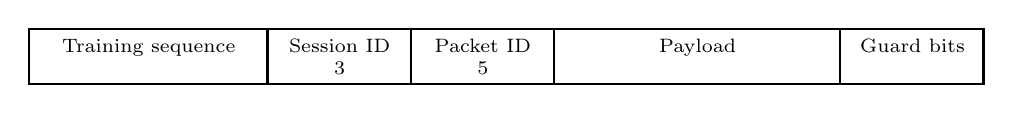
\begin{tikzpicture}[                
                    slot/.style={
            		text centered,
			font=\scriptsize,
			align=center,
			anchor=center,
			minimum height=0.7cm
            	}]
\draw[thick] (0,0) rectangle (\linewidth, -0.7);
\draw[thick] (0.25\linewidth,0) -- ++(0, -0.7);
\draw[thick] (0.4\linewidth,0) -- ++(0, -0.7);
\draw[thick] (0.55\linewidth,0) -- ++(0, -0.7);
\draw[thick] (0.85\linewidth,0) -- ++(0, -0.7);

\draw
(0,0) node[slot, minimum width=0.25\linewidth, anchor=north west](barker){Training sequence \\ \barkerBitsQPSK}
(0.25\linewidth,0)  node[slot, minimum width=0.15\linewidth, anchor=north west](barker){Session ID \\ 3}
(0.4\linewidth,0)  node[slot, minimum width=0.15\linewidth, anchor=north west](barker){Packet ID \\ 5}
(0.55\linewidth,0) node[slot, minimum width=0.30\linewidth, anchor=north west](barker){Payload \\ \packetDataBitsQPSK}
(0.85\linewidth,0) node[slot, minimum width=0.15\linewidth, anchor=north west](barker){Guard bits \\ \guardBitsQPSK}
;	

\end{tikzpicture}
}
  \\
  \subfloat[QAM-16 data packet\label{1b}]{%
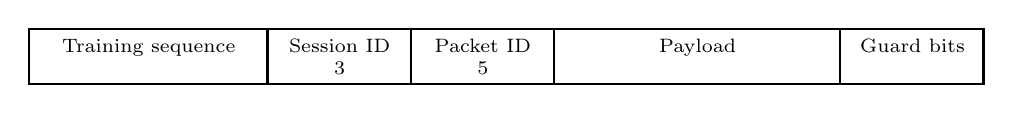
\begin{tikzpicture}[                
                    slot/.style={
            		text centered,
			font=\scriptsize,
			align=center,
			anchor=center,
			minimum height=0.7cm
            	}]
\draw[thick] (0,0) rectangle (\linewidth, -0.7);
\draw[thick] (0.25\linewidth,0) -- ++(0, -0.7);
\draw[thick] (0.4\linewidth,0) -- ++(0, -0.7);
\draw[thick] (0.55\linewidth,0) -- ++(0, -0.7);
\draw[thick] (0.85\linewidth,0) -- ++(0, -0.7);

\draw
(0,0) node[slot, minimum width=0.25\linewidth, anchor=north west](barker){Training sequence \\ \barkerBitsQAM}
(0.25\linewidth,0)  node[slot, minimum width=0.15\linewidth, anchor=north west](barker){Session ID \\ 3}
(0.4\linewidth,0)  node[slot, minimum width=0.15\linewidth, anchor=north west](barker){Packet ID \\ 5}
(0.55\linewidth,0) node[slot, minimum width=0.30\linewidth, anchor=north west](barker){Payload \\ \packetDataBitsQAM}
(0.85\linewidth,0) node[slot, minimum width=0.15\linewidth, anchor=north west](barker){Guard bits \\ \guardBitsQAM}
;	

\end{tikzpicture}}
\\
  \subfloat[QPSK BER packet\label{1c}]{%
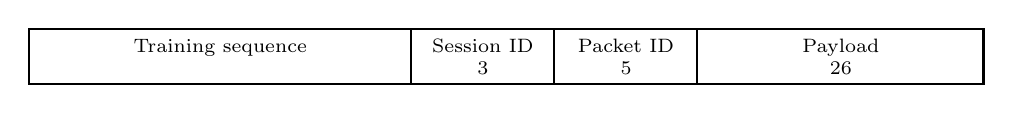
\begin{tikzpicture}[                
                    slot/.style={
            		text centered,
			font=\scriptsize,
			align=center,
			anchor=center,
			minimum height=0.7cm
            	}]
\draw[thick] (0,0) rectangle (\linewidth, -0.7);
\draw[thick] (0.40\linewidth,0) -- ++(0, -0.7);
\draw[thick] (0.55\linewidth,0) -- ++(0, -0.7);
\draw[thick] (0.70\linewidth,0) -- ++(0, -0.7);

\draw
(0,0) node[slot, minimum width=0.4\linewidth, anchor=north west](barker){Training sequence \\ \barkerBitsQPSK}
(0.40\linewidth,0)  node[slot, minimum width=0.15\linewidth, anchor=north west](barker){Session ID \\ 3}
(0.55\linewidth,0)  node[slot, minimum width=0.15\linewidth, anchor=north west](barker){Packet ID \\ 5}
(0.7\linewidth,0) node[slot, minimum width=0.3\linewidth, anchor=north west](barker){Payload \\ 26}
;	

\end{tikzpicture}}
  \caption{Burst format (bits) for QPSK(a) and QAM-16(b) modulated data packets, and QPSK modulated BER packet (c)}
  \label{fig:burst_format} 
\end{figure}
 